% TIPO DE DOCUMENTO
\documentclass[12pt]{article}

% region PAQUETES QUE VAMOS A USAR
\usepackage{amsmath}
\usepackage{amssymb} 
\usepackage[utf8]{inputenc} 
\usepackage[spanish]{babel} 
\usepackage{comment}
\usepackage{graphicx}
\usepackage{wrapfig}
\usepackage{float}
\usepackage{xcolor}
\usepackage{tikz}
\usepackage{emptypage}
\usepackage{geometry}
\usepackage{amsthm}
\usepackage{url}
\usepackage[colorlinks=true,linkcolor=]{hyperref}
\usepackage[all]{xy}
\usepackage{fancyhdr}
\usepackage{pdfpages}
\usepackage{lipsum}
\usepackage{fix-cm}
\usepackage{yhmath}
\usepackage{multimedia}
% endregion

\usetikzlibrary{calc, arrows.meta, babel}

% --- CONFIGURACIÓN DE ESPACIADO ENTRE PÁRRAFOS ---
% Esto añade exactamente 1mm de espacio cada vez que dejas una línea en blanco (nuevo párrafo)
\setlength{\parskip}{2mm}

% region ABREVIATURAS
\newcommand{\N}{\mathbb{N}}
\newcommand{\R}{\mathbb{R}}
\newcommand{\F}{\mathcal{F}}
\newcommand{\A}{\mathcal{A}}
% endregion

% region DEFINIMOS LOS ENTORNOS
\theoremstyle{definition}
\newtheorem{definicion}{\textbf{Definición}}[section]
\newtheorem{nota}{Nota}[section]
\newtheorem*{nota*}{Nota}
\theoremstyle{plain}
\newtheorem{teorema}{Teorema}[section]
\newtheorem*{teorema*}{Teorema}
\theoremstyle{plain}
\newtheorem{propiedad}{Propiedades}[section]
\theoremstyle{definition}
\newtheorem{definiciones}{Definiciones}[section]
% endregion

% --- MODIFICACIÓN DEL TÍTULO DEL ÍNDICE ---
\renewcommand{\contentsname}{Índice General}

% MÁRGENES DESEADOS
\geometry{a4paper,left=2cm,right=2cm,top=2cm,bottom=2cm}

% --- ARREGLO PARA FANCYHDR ---
\setlength{\headheight}{16pt} 

% INDENTACION
\setlength{\parindent}{0pt} 

%%%%%%%%%%%%%%%%%%%%%%%%%%%%%%%%%%%%%%%%%%%%%%%%%%%%%%%%
%%%%%%%% variables de la cabecera %%%%%%%%%%%%%%%%%%%%%
%%%%%%%%%%%%%%%%%%%%%%%%%%%%%%%%%%%%%%%%%%%%%%%%%%%%%%%

\newcommand{\tituloacademico}{Grado en Matemáticas}

\newcommand{\documento}{TRABAJO ESTADÍSTICA\\
COMBINATORIA}

\newcommand{\fechatrabajo}{Mayo 2026}
\newcommand{\autor}{Isabel Llera Martínez\\
                    Álvaro Rivero Horrillo}

% -------------------------------------------------------------------------------------------------------------------------------------------%

\begin{document}

%\begin{titlepage}
% Lado izqdo. de la p\'agina
\begin{minipage}{0.20\textwidth}
\begin{flushleft}
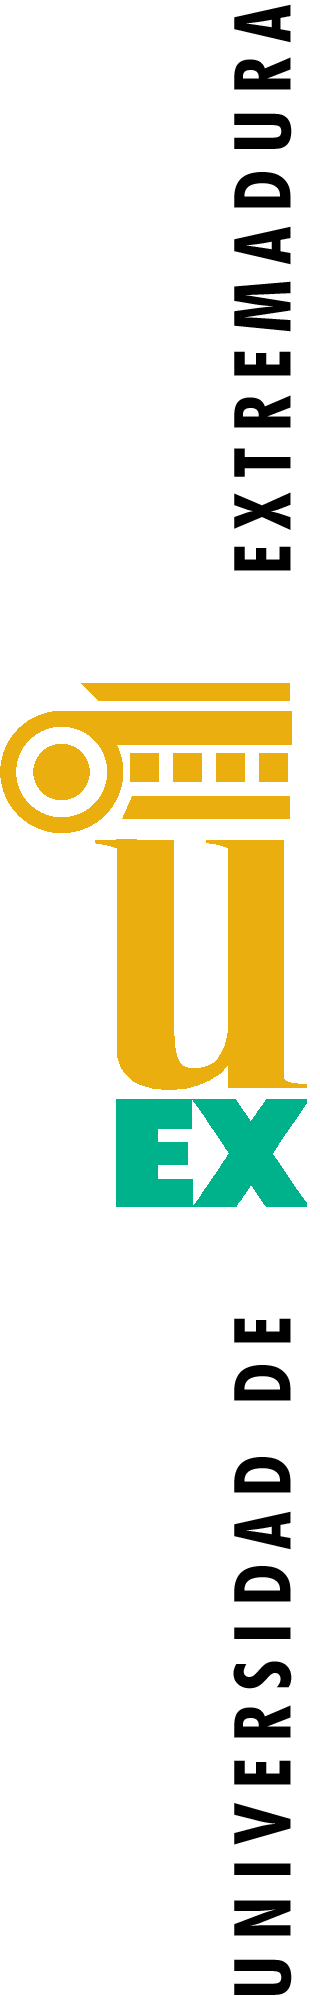
\includegraphics[scale=0.3, width=3cm]{./logos/marca_UEx_4_color.png}
\end{flushleft}
\end{minipage}
% Lado derecho de la p\'agina
\begin{minipage}{0.78\textwidth}

\vspace{3cm}

\centering
    \textsc{\LARGE Facultad de Ciencias}\\[1cm]
    \textsc{\Large \tituloacademico}\\[2cm]

\centering
    \textsc{\large \documento}\\[3cm]

\flushright
\textsc{\normalsize \autor}\\

\vspace{10mm}

\textsc{\normalsize \fechatrabajo}\\
\end{minipage}

\end{titlepage}

\tableofcontents

\newpage 

\pagestyle{plain} 

\section{Introducción}

La combinatoria es una rama fundamental de las matemáticas que se ocupa del estudio de las diversas formas de organizar y contar los elementos de un conjunto bajo restricciones específicas. Centrándose en relaciones lógicas y estructurales entre los elementos, independientemente de su naturaleza física.

El desarrollo formal de la combinatoria moderna se remonta al siglo XVII con los estudios sobre probabilidad de Fermat y Pascal. Siendo este último, el primero en establecer la relación intrínseca que existe entre los números combinatorios y el desarrollo de las potencias de un binomio, popularizando lo que hoy se conoce como el Triángulo de Pascal.

De forma simultánea, será Leibniz, quién, en 1666, sentará las bases teóricas de las permutaciones y combinaciones. No obstante, el salto hacia una teoría general lo dará  Bernoulli, pues fue él quien sistematizó el uso de las combinaciones aplicadas al cálculo de probabilidades y quien demostró formalmente  el Teorema binomial para exponentes enteros positivos:

\begin{equation*}
    (a+b)^n = \sum_{k=0}^{n} \binom{n}{k} a^{n-k}b^k
\end{equation*}

Posteriormente, fue Euler quien expande los horizontes de la disciplina mediante el estudio de las particiones de números enteros (escribir un número natural como suma de otros), introduciendo el uso de las funciones generatrices, una herramienta que transformó la combinatoria en una disciplina con métodos analíticos profundos.

Finalmente, cabe destacar que, la combinatoria experimentó una transformación profunda en el siglo XX. Gracias a figuras como Erdös, pasó de ser una  colección de problemas aislados a convertirse en una disciplina central de la matemática moderna, con aplicaciones cruciales en la informática teórica, la optimización y la teoría de grafos.



\section{Técnicas básicas de recuento}

    \subsection{Principio de Adición}
    \subsection{Principio de Multiplicación}
    \subsection{Principio del Palomar}
    \subsection{Principio de Inclusión-Exclusión o Principio de la Criba}

\section{Combinatoria}

    \subsection{Número factorial}
    \subsection{Número combinatorio y sus propiedades}
    \subsection{Triángulo de Pascal}

\section{Permutaciones}

    \subsection{Permutaciones sin repetición}
    \subsection{Permutaciones circulares}
    \subsection{Permutaciones con repetición}

\section{Variaciones}

    \subsection{Variaciones sin repetición}
    \subsection{Variaciones con repetición}

\section{Combinaciones}

    \subsection{Combinaciones sin repetición}
    \subsection{Combinaciones con repetición}

\section{Resumen}

\newpage

\section{Conclusión}

% Elige el estilo de la bibliografía (plain, alpha, apalike, ieeetr, etc.)

\nocite{*}
\bibliographystyle{plain} 

% % Llama a tu archivo .bib (sin la extensión .bib)
\bibliography{bibliografia}

\end{document}